\documentclass[11pt,fleqn, a4paper]{exam}
\usepackage[utf8]{inputenc}

\usepackage[margin=1in]{geometry}
\usepackage{amsmath,amssymb}
\usepackage{gensymb}
\usepackage{multicol}
\usepackage{float}
\usepackage{graphicx}
\usepackage{units,icomma}
\usepackage{hyperref}
\usepackage{enumerate}
\usepackage{wasysym}
\usepackage{multirow}
\usepackage[usenames,dvipsnames]{xcolor}
\usepackage[margin=1.5cm]{caption}
%\everymath{\displaystyle}

\hyphenation{
  chro-no-ampe-ro-met-ric
  ber-dia-me-ter
  de-ngan
  me-nem-pati
  mic-ro-graphs}

\renewcommand{\figurename}{Gambar.}
\renewcommand{\labelitemi}{$-$}


\newcommand{\class}{OLIMPIADE ASTRONOMI}
\newcommand{\term}{Tingkat Kabupaten/Kota - 2016}
\newcommand{\examnum}{OSK Astronomi 2016}
%\newcommand{\examdate}{11/02/2014}
%\newcommand{\timelimit}{120 Minutes}

\pagestyle{head}
\firstpageheader{}{}{}
\runningheader{\examnum}{}{Halaman \thepage\ dari \numpages}
\runningheadrule


\begin{document}

\noindent
\begin{tabular*}{\textwidth}{l @{\extracolsep{\fill}} r @{\extracolsep{6pt}} l}
\textbf{\class} \\% & \textbf{Name:} & \makebox[2in]{\hrulefill}\\
\textbf{\term}  %&&\\
%\textbf{\examnum} &&\\
%\textbf{\examdate} &&\\
%\textbf{Time Limit: \timelimit} & Teaching Assistant & \makebox[2in]{\hrulefill}
\end{tabular*}\\
\rule[2ex]{\textwidth}{2pt}

\noindent
\begin{tabular}{ll}
\textit{Copyright} (c) 2016 & Ridlo W. Wibowo (ridlo.w.wibowo@gmail.com)\\
                   & Sulistiyowati (sulis.astro08@gmail.com)
\end{tabular}

\vspace{0.3cm}
\noindent
Solusi ini dibuat tanpa jaminan kesesuaian dengan solusi resmi dari juri olimpiade sains bidang Astronomi. Pengguna boleh menyebarluaskan dan/atau memodifikasi solusi ini dengan mencantumkan sumber asli. Hak cipta soal ada pada Kementerian Pendidikan dan Kebudayaan dan dilindungi undang-undang.

\vspace{0.4cm}
\noindent
\rule[2ex]{\textwidth}{1.5pt}

\textbf{Soal Pilihan Berganda}

\begin{questions}
\question Assume that Earth revolves around the Sun with a circular orbit and its distance is 1 au. The equation which describes Earth's position in cartesian coordinates relative to the Sun is
\begin{choices}
\choice $y=x$
\choice $y=1-x$
\choice $y=1+x^2$
\choice $y^2=1-x^2$
\choice $(x-1)^{2} + (y-1)^{2} = 1$
\end{choices}

\textit{Jawaban: D}\\
Posisi Bumi relatif terhadap Matahari artinya Matahari dijadikan sebagai `pusat koordinat'. Persamaan lingkaran dengan pusat di (0, 0) dan radius 1 adalah
\begin{eqnarray*}
x^2 + y^2 &=& 1^2\\
y^2 &=& 1 - x^2
\end{eqnarray*}


\vspace{0.5cm}
\question Diketahui 
\begin{equation*}
y^2 = r^2 \left( \tan^{2}{c} + \tan^{2}{b} - 2 \tan{b} \tan{c} \cos{A} \right)
\end{equation*}
dan
\begin{equation*}
y^2 = r^2 \left( \sec^{2}{c} + \sec^{2}{b} - 2 \sec{b} \sec{c} \cos{a} \right)
\end{equation*}
Dari kedua persamaan tersebut dapat diperoleh

\begin{choices}
\choice $\cos{b} = \cos{c} \cos{a} + \sin{c} \sin{a} \cos{B}$
\choice $\cos{a} = \cos{b} \cos{c} + \sin{b} \sin{c} \cos{A}$
\choice $\cos{c} = \cos{a} \cos{b} + \sin{a} \sin{b} \cos{C}$
\choice $\sin{a} = \sin{b} \sin{c} + \cos{b} \cos{c} \cos{A}$
\choice $\cos{a} = -\tan{b} \tan{c}$
\end{choices}

\textit{Jawaban: B}\\
Kedua persamaan di atas memberikan hubungan
\begin{equation*}
\tan^{2}{c} + \tan^{2}{b} - 2 \tan{b} \tan{c} \cos{A} = \sec^{2}{c} + \sec^{2}{b} - 2 \sec{b} \sec{c} \cos{a}
\end{equation*}
dengan menggunakan hubungan $\sec^{2}{x} = 1 + \tan^{2}{x}$ dapat diperoleh 
\begin{eqnarray*}
\tan^{2}{c} + \tan^{2}{b} - 2 \tan{b} \tan{c} \cos{A} &=& 2 + \tan^{2}{c} + \tan^{2}{b} - 2 \sec{b} \sec{c} \cos{a}\\
- 2 \tan{b} \tan{c} \cos{A} &=& 2 - 2 \sec{b} \sec{c} \cos{a}\\
- \frac{\sin{b} \sin{c} \cos{A}}{\cos{b} \cos{c}} &=& 1 - \frac{\cos{a}}{\cos{b} \cos{c}}\\
\cos{b} \cos{c} - \cos{a} &=& - \sin{b} \sin{c} \cos{A}\\
\cos{a} &=& \cos{b} \cos{c} + \sin{b} \sin{c} \cos{A}
\end{eqnarray*}


\vspace{0.5cm}
\question An astronomer measured diameter of some asteroids. From her measurement, she created a histogram as you can find in the following. What are the median and the mode of the data?
\begin{figure}[H]
\centering
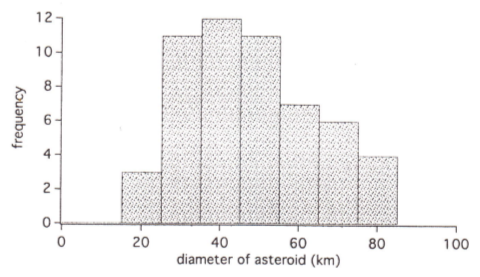
\includegraphics[width=0.6\textwidth]{gambar/osk2016_3.png}
\end{figure}
\begin{choices}
\choice 12 and 40
\choice 50 and 50
\choice 50 and 40
\choice 40 and 50
\choice 40 and 40
\end{choices}

\textit{Jawaban: C}\\
Data yang disajikan sepertinya merupakan data tunggal (bukan data berkelompok). Nilai median (nilai tengah) dapat ditentukan dengan mengurutkan data lalu mencari di mana titik tengahnya.
\begin{table}[H]
\centering
\begin{tabular}{|c|c|}
\hline 
Diameter asteroid & Frekuensi \\ 
\hline 
20 & 3 \\ 
\hline 
30 & 11 \\ 
\hline 
40 & 12 \\ 
\hline 
50 & 11 \\ 
\hline 
60 & 7 \\ 
\hline 
70 & 6 \\ 
\hline 
80 & 4 \\ 
\hline 
Jumlah asteroid & 54 \\ 
\hline 
\end{tabular} 
\end{table}

Karena data berjumlah genap ($N = 54$), maka dapat kita rata-ratakan nilai ke $\frac{N}{2} = 27$ yaitu 50 dan nilai ke $\frac{N}{2}+1 = 28$ yaitu 50, sehingga
\begin{eqnarray*}
\text{median} = \frac{50 + 50}{2} = 50
\end{eqnarray*}

Mode adalah nilai yang paling sering keluar pada sekumpulan data. Modus/Mode dari data di atas adalah 40 (frekuensinya paling besar).


\vspace{0.5cm}
\question Sebuah sensor kamera berbentuk persegi panjang dengan luas sebesar 130 cm$^{2}$. Jika panjang sensor kamera tersebut 7 cm lebih pendek dari dua kali lebarnya, maka lebarnya adalah
\begin{choices}
\choice 6,0 cm
\choice 6,5 cm
\choice 10,0 cm
\choice 12,0 cm
\choice 15,0 cm
\end{choices}

\textit{Jawaban: C}\\
Persamaan luas persegi panjang
\begin{equation*}
p \cdot l = 130
\end{equation*}
Hubungan panjang dan lebar diberikan sebagai
\begin{eqnarray*}
2l - p &=& 7\\
2l - 130/l &=& 7\\
2l^{2} - 7l - 130 &=& 0\\
\end{eqnarray*}
Solusi dari persamaan kuadrat di atas dapat dicari dengan persamaan ``\textit{abc}'',
\begin{eqnarray*}
l_{12} = \frac{7 \pm \sqrt{49 + 1040}}{4}
\end{eqnarray*}
menghasilkan nilai $l_1 = 10$ dan $l_2 = -6.5$. Dapat disimpulkan lebar sensor kamera tersebut adalah 10 cm.


\vspace{0.5cm}
\question Hipparchus menentukan magnitudo bintang sebagai skala logaritmik untuk menggambarkan terang bintang relatif terhadap bintang lainnya. Magnitudo bintang dapat ditentukan menggunakan rumus
\begin{equation*}
m = -2,5 \log{E} + C
\end{equation*}
dengan $m$, $E$, dan $C$ masing-masing adalah magnitudo bintang, fluks energi bintang yang diterima di Bumi, dan tetapan. Nilai $E$ pada bintang A dan bintang B masing-masing adalah $E = 3 \times 10^{-5}$ J/s/m$^2$ dan $E = 7 \times 10^{-7}$ J/s/m$^2$. Jika bintang A mempunyai magnitudo 4, maka magnitudo bintang B adalah  

\begin{choices}
\choice 0
\choice 6
\choice 8
\choice 9
\choice 15
\end{choices}

\textit{Jawaban: C}
\begin{eqnarray*}
m_B-m_A&=&-2,5\log E_B+C - (-2,5\log E_A+C)\\
m_B-m_A&=&-2,5\log \frac{E_B}{E_A} \\
m_B-m_A&=&-2,5\log \frac{7 \times 10^{-7}}{3 \times 10^{-5}} \\
m_B-m_A&=&4.08\\
m_B&=&8.08\\
\end{eqnarray*}
 

\vspace{0.5cm}
\question Deklinasi Matahari $y$ sebagai fungsi waktu $t$ dapat dinyatakan sebagai 
\begin{equation*}
y = 23,5^{\circ} \sin{\left( \frac{2\pi(t-80)}{T} \right)}
\end{equation*}
dengan $t$ adalah jumlah hari sejak 1 Januari pada tahun bukan kabisat, dan $T$ adalah periode revolusi Bumi 365,25 hari. Pada tanggal berapakah $y$ bernilai maksimum dan minimum?
\begin{choices}
\choice 21 Maret dan 23 September
\choice 22 Juni dan 22 Desember
\choice 21 Maret dan 22 Desember
\choice 21 Juni dan 20 Desember
\choice 1 Januari dan 1 Agustus
\end{choices}

\textit{Jawaban: D}\\
Persamaan tersebut memberikan nilai maksimum dan minimum ketika argumen $\sin$ pada ruas kanan maksimum dan minimum juga (ingat bahwa nilai $\sin$ selalu dalam rentang -1 hingga 1). Nilai maksimum terjadi untuk $\sin{\frac{\pi}{2}}$ dan minimum untuk $\sin{\frac{3\pi}{2}}$.

Saat maksimum 
\begin{eqnarray*}
\frac{2\pi(t-80)}{365,25} &=& \frac{\pi}{2}\\
t - 80 &=& 91,3125\\
t &=& 171,3125 \quad \text{(172) hari semenjak 1 Januari = 21 Juni}
\end{eqnarray*}
Saat minimum
\begin{eqnarray*}
\frac{2\pi(t-80)}{365,25} &=& \frac{3\pi}{2}\\
t - 80 &=& 273,9375\\
t &=& 353,9375 \quad \text{(354) hari semenjak 1 Januari = 20 Desember}
\end{eqnarray*}


\vspace{0.5cm}
\question Jarak planet-planet dari Matahari dalam satuan astronomi ternyata mempunyai pola:
\begin{equation*}
\frac{7}{10}, \frac{10}{10}, \frac{16}{10}, \frac{28}{10}, \frac{52}{10}, \dots 
\end{equation*}
Formula jarak $r$ untuk baris bilangan tersebut adalah
\begin{choices}
\choice $r = 2n + 0,4$ dengan $n = 1, 2, 3, 4, \dots$
\choice $r = (3n + 2)/10$ dengan $n = 0, 1, 2, 3, \dots$
\choice $r = (n^2 + 0,4)/10$ dengan $n = 1, 2, 3, 4, \dots$
\choice $r = (3 \times 2^n + 4)/10$ dengan $n = 0, 1, 2, 3, \dots$
\choice $r = (2n + 1) \times 0,1$ dengan $n = 1, 2, 3, 4, \dots$
\end{choices}

\textit{Jawaban: D}\\
Sesuai dengan pola.


\vspace{0.5cm}
\question Di sebuah eksoplanet, terdapat organisme sejumlah
\begin{equation*}
N_{\text{awal}} = \frac{\log{b^2}}{\log{a}}
\end{equation*}
Dalam seabad, jumlah tersebut meningkat $^{b}\log{c}$ kali. Kemudian, jumlahnya berkurang sebesar $^{a}\log{\frac{1}{c}}$ karena bencana. Jika $a$, $b$, dan $c$ merupakan bilangan positif, organisme yang tersisa adalah
\begin{choices}
\choice $N_{\text{akhir}} = 0$
\choice $N_{\text{akhir}} = 1$
\choice $N_{\text{akhir}} = ^{a}\log{b^2}$
\choice $N_{\text{akhir}} = 2 \cdot ^{b}\log{c}$
\choice $N_{\text{akhir}} = 3 \cdot ^{a}\log{c}$
\end{choices}

\textit{Jawaban: E}\\
Meningkat $^{b}\log{c}$ kali, lalu berkurang $^{a}\log{\frac{1}{c}}$
\begin{eqnarray*}
N_{\text{akhir}} &=& \frac{\log{b^2}}{\log{a}} \cdot ^{b}\log{c} - ^{a}\log{\frac{1}{c}}\\
&=& ^{a}\log{b^2} \cdot ^{b}\log{c} - ^{a}\log{c^{-1}}\\
&=& 2 \cdot ^{a}\log{b} \cdot ^{b}\log{c} + ^{a}\log{c}\\
&=& 2 \cdot ^{a}\log{c} + ^{a}\log{c}\\
&=& 3 \cdot ^{a}\log{c}
\end{eqnarray*}

\vspace{0.5cm}
\question  Di dekat sebuah gunung api, ditemukan bakteri yang tahan terhadap panas (termofilik). Awalnya terdapat 75 bakteri dalam gelas ukur 1 liter. Bakteri tersebut terus-menerus membelah diri menjadi dua tiap 100 detik. Setelah didiamkan selama 75 menit, gelas terisi penuh. Berapakah volume rata-rata bakteri tersebut?
\begin{choices}
\choice $5,68 \times 10^{-14} $ ml
\choice $2,30 \times 10^{-14} $ ml
\choice $3,79 \times 10^{-16} $ ml
\choice $7,58 \times 10^{-16} $ ml
\choice $1,89 \times 10^{-16} $ ml
\end{choices}

\textit{Jawaban:} Tidak ada; \textit{C} jika satuannya liter\\
Selama 75 menit terjadi pembelahan sejumlah 
\begin{equation*}
n = \frac{75 \times 60}{100} = 45 \quad \text{kali}
\end{equation*}
Penambahan jumlah bakteri membentuk deret geometri
\begin{equation*}
a, ar, ar^2, ar^3, \dots
\end{equation*}
dengan $a = 75$ dan $r = 2$. Pembelahan terjadi sebanyak 45 kali sehingga jumlahnya menjadi
\begin{equation*}
N = 75 \times 2^{45} = 2,64 \times 10^{15} \quad \text{bakteri}
\end{equation*}
Volume rata-rata bakteri 
\begin{equation*}
\overline{V} = \frac{1000}{2,64 \times 10^{15}} = 3,79 \times 10^{-13} \quad \text{ml}
\end{equation*}


\vspace{0.5cm}
\question Dalam tata koordinat kartesian, sebuah komet memiliki lintasan parabola dengan persamaan
\begin{equation*}
f(x) = x^2 - 11x + 28
\end{equation*}
Sementara itu, suatu benda tak dikenal melintasi Tata Surya dengan lintasan berupa garis lurus yang memenuhi persamaan
\begin{equation*}
4x + 7y - 60 = 0
\end{equation*}
Kedua benda dapat bertabrakan di titik
\begin{choices}
\choice (2, 10)
\choice (2, 7)
\choice (3, 4)
\choice (8, 4)
\choice Tidak ada titik perpotongan
\end{choices}

\textit{Jawaban: D}\\
Asumsi pertama untuk menjawab permasalahan ini yaitu pada persamaan pertama berlaku $f(x) = y$. Jika asumsi itu tidak berlaku, maka jawabannya bisa jadi tidak terdapat titik potong antar kedua kurva. Selanjutnya jika kita gunakan asumsi kedua kurva sebidang tersebut, maka permasalahan di atas berubah menjadi permasalahan mencari titik potong antara dua kurva, 
\begin{eqnarray*}
x^2 - 11x + 28 &=& -\frac{4}{7} x + \frac{60}{7}\\
x^2 - \frac{73}{7}x + \frac{136}{7} &=& 0\\
7x^2 - 73 + 136 &=& 0
\end{eqnarray*}
Solusi dari persamaan di atas adalah
\begin{eqnarray*}
x_{12} &=& \frac{73 \pm \sqrt{73^2 - 4 \cdot 7 \cdot 136}}{2 \cdot 7}\\
x_{12} &=& \frac{73 \pm \sqrt{1521}}{14}\\
x_{12} &=& \frac{73 \pm 39}{14}\\
x_{1} &=& 8 \quad x_{2} = 2,4286
\end{eqnarray*}
Dapat kita coba untuk nilai $x = 8$, maka kedua persamaan terpenuhi dengan nilai $y$ yang sama 
$$y = 8^2 - 11 \cdot 8 + 28 = 4$$
$$y = -\frac{4}{7} \cdot 8 + \frac{60}{7} = 4$$
\begin{figure}[H]
\centering
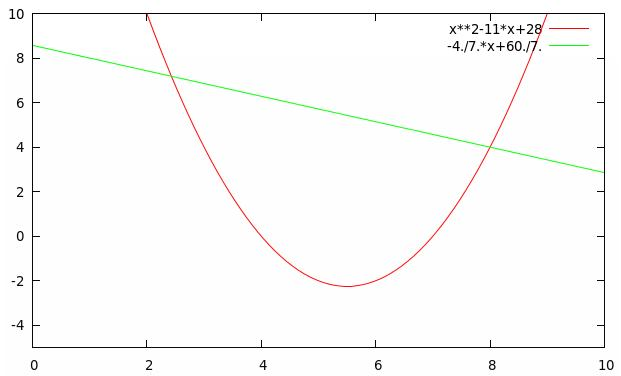
\includegraphics[width=0.7\textwidth]{gambar/osk2016_10.jpg}
\end{figure}

\vspace{0.5cm}
\question Pada suatu saat, komet ISON teramati berada pada jarak 2,0 sa dengan sudut $135^{\circ}$ dari arah Matahari, maka jarak komet ISON dari Matahari saat itu adalah
\begin{choices}
\choice 2,8 sa
\choice 3,6 sa
\choice 5,0 sa
\choice 5,3 sa
\choice 6,4 sa
\end{choices}

\textit{Jawaban: A}
\begin{figure}[H]
\centering
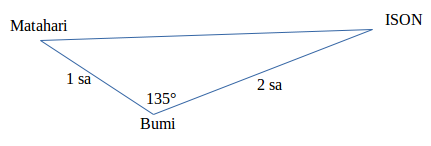
\includegraphics[width=0.6\textwidth]{gambar/osk2016_11.png}
\end{figure}

Jarak Matahari-ISON dapat ditentukan dengan persamaan \textit{cosinus}
\begin{eqnarray*}
d^2 &=& 1^2 + 2^2 - 2 \cdot 1 \cdot 2 \cdot \cos{135^{\circ}}\\
d &=& 2,8 \quad \text{sa} 
\end{eqnarray*}

\vspace{0.5cm}
\question Diketahui bahwa gaya $\overrightarrow{F_1} = (2\hat{i} + 4\hat{j})$ N dan gaya $\overrightarrow{F_2} = (3\hat{i} + \hat{j})$ N. Jika kedua gaya tersebut membentuk sudut $45^{\circ}$, maka besar resultan kedua gaya tersebut adalah
\begin{choices}
\choice $5 $ N
\choice $5 \sqrt{2} $ N
\choice $\sqrt{10} $ N
\choice $2 \sqrt{5} $ N
\choice $10 \sqrt{2} $ N
\end{choices}

\textit{Jawaban: B}\\
Soal ini memberikan informasi yang berlebih, dua gaya sudah diberikan dalam bentuk vektor di koordinat kartesian, akan tetapi informasi kedua memberikan besar sudut antar keduanya yang sebenarnya tidak perlu.
Sudut antara dua vektor tersebut sudah terkandung pada informasi pertama
\begin{eqnarray*}
\overrightarrow{F_1} \bullet \overrightarrow{F_2} &=& \Vert \overrightarrow{F_1} \Vert \Vert \overrightarrow{F_2} \Vert \cos{\theta}\\
(2 \cdot 3) + (4 \cdot 1) &=& \sqrt{20} \sqrt{10} \cos{\theta}\\
10 &=& \sqrt{200} \cos{\theta}\\
\cos{\theta} &=& \sqrt{\frac{1}{2}} = \frac{1}{2} \sqrt{2}\\
\theta &=& 45^{\circ}
\end{eqnarray*}
Resultan dua gaya tersebut adalah
\begin{eqnarray*}
\overrightarrow{R} &=& \overrightarrow{F_1} + \overrightarrow{F_2}\\
\overrightarrow{R} &=& (2\hat{i} + 4\hat{j}) + (3\hat{i} + \hat{j})\\
\overrightarrow{R} &=& 5\hat{i} + 5\hat{j}\\
\Vert \overrightarrow{R} \Vert &=& \sqrt{5^2 + 5^2} = \sqrt{50} = 5\sqrt{2} \quad \text{N}
\end{eqnarray*}

\vspace{0.5cm}
\question Diketahui massa dan radius planet Neptunus masing-masing adalah $1,024 \times 10^{26}$ kg dan $2,462 \times 10^7$ m. Berapa berat sebuah objek di planet Neptunus jika diketahui massanya di Bulan adalah sebesar 930 kg?
\begin{choices}
\choice 10478 N 
\choice 1048 N
\choice 105 N
\choice 6341 N
\choice 63409 N
\end{choices}

\textit{Jawaban: A}\\
Massa selalu tetap, tidak bergantung pada percepatan gravitasi. Berat bergantung pada besarnya percepatan gravitasi.
\begin{eqnarray*}
W &=& m \cdot g\\
W &=& 930 \cdot \frac{GM_{\text{Nept}}}{R_{\text{Nept}}^{2}}\\
W &=& 930 \cdot 11,268\\
W &=& 10479,3 \quad N  
\end{eqnarray*}
 

\vspace{0.5cm}
\question Terdapat asteroid A dan B dengan massa asteroid A dua kali lebih besar dari B. Awalnya asteroid A dalam keadaan diam dan asteroid B bergerak menuju asteroid A dengan kecepatan 2 km/s. Setelah tumbukan asteroid A bergerak 1/5 kali kecepatan awal asteroid B. Kecepatan asteroid B setelah tumbukan adalah
\begin{choices}
\choice 1,9 km/s
\choice 720 km/jam
\choice 900 m/s
\choice 4320 km/jam
\choice Tidak dapat ditentukan dengan informasi yang diberikan
\end{choices}

\textit{Jawaban: D} \\
Diketahui $m_A = 2 m_B$, $v_{Af} = \frac{1}{5} v_{Bi} = 400$ m/s.

Kita gunakan hukum kekekalan momentum,
\begin{eqnarray*}
m_A v_{Ai} + m_B v_{Bi} &=& m_A v_{Af} + m_B v_{Bf}\\
2 m_B \cdot 0 + m_B \cdot 2000 &=& 2 \cdot m_B \cdot 400 + m_B \cdot v_{Bf}\\
v_{Bf} &=& \frac{2000 m_B - 800 m_B}{m_B}\\
v_{Bf} &=& 1200 \quad \text{m/s} = 4320 \quad \text{km/jam}
\end{eqnarray*}
Kita dapat lakukan pengecekan apakah masalah tumbukan di atas memenuhi hukum kekekalan energi kinetik. Jika total energi kinetik setelah tumbukan $\leq$ total energi kinetik sebelum tumbukan, maka solusi tersebut dapat diterima. Jika tidak, maka kemunginan masih ada yang salah dengan data yang diberikan.

Total energi kinetik sebelum tumbukan
\begin{equation*}
E_{i} = \frac{1}{2} m_A v_{Ai}^2 + \frac{1}{2} m_B v_{Bi}^2 = \frac{1}{2} m_B 2000^2 = \frac{1}{2} m_B \cdot 4 \times 10^6
\end{equation*}
Total energi kinetik setelah tumbukan
\begin{eqnarray*}
E_{f} &=& \frac{1}{2} m_A v_{Af}^2 + \frac{1}{2} m_B v_{Bf}^2 = \frac{1}{2} m_A \cdot 400^2 + \frac{1}{2} m_B \cdot 1200^2\\ 
&=& \frac{1}{2} m_B \cdot (2 \cdot 400^2 + 1200^2)\\
&=& \frac{1}{2} m_B \cdot 1,76 \times 10^6
\end{eqnarray*}
Karena total energi kinetik setelah tumbukan lebih kecil dari sebelum tumbukan, maka hasil di atas ``sah'' dan termasuk dalam jenis tumbukan tidak elastis.

%Hukum kekekalan momentum
%\begin{equation}
%\label{eq:momentum}
%m_1 v_{1i} + m_2 v_{2i} = m_1 v_{1f} + m_2 v_{2f}
%\end{equation}
%Hukum kekekalan energi kinetik
%\begin{equation}
%\label{eq:kinetik}
%\frac{1}{2} m_1 v_{1i}^2 + \frac{1}{2} m_2 v_{2i}^2 = \frac{1}{2} m_1 v_{1f}^2 + \frac{1}{2} m_2 v_{2f}^2
%\end{equation}
%Pers. \eqref{eq:momentum} memberikan hubungan
%\begin{equation}
%m_1 (v_{1i} - v_{1f}) = m_2 (v_{2f} - v_{2i})
%\end{equation}
%Pers. \eqref{eq:kinetik} memberikan hubungan lain
%\begin{eqnarray}
%m_1 v_{1i}^2 + m_2 v_{2i}^2 &=& m_1 v_{1f}^2 + m_2 v_{2f}^2\\
%m_1 (v_{1i}^2 - v_{1f}^2) &=& m_2 (v_{2f}^2 - v_{2i}^2)\\
%m_1 (v_{1i} + v_{1f}) (v_{1i} - v_{1f}) &=& m_2 (v_{2f} + v_{2i}) (v_{2f} - v_{2i})
%\end{eqnarray}
%Dengan membagi Pers. (6) dengan Pers. (3) kita dapatkan
%\begin{eqnarray*}
%v_{1i} + v_{1f} &=& v_{2f} + v_{2i}\\
%v_{1i} - v_{2i} &=& -(v_{1f} - v_{2f})
%\end{eqnarray*}
%Hubungan di atas dan Pers. \eqref{eq:momentum} dapat digunakan untuk menyelesaikan kasus-kasus tumbukan elastis sempurna. Misalkan saja jika diketahui kedua massa dan kecepatan awalnya, maka dapat kita turunkan kecepatan akhir masing-masing benda adalah
%\begin{eqnarray*}
%v_{1f} &=& \frac{m_1 - m_2}{m_1 + m_2} v_{1i} + \frac{2 m_2}{m_1 + m_2} v_{2i}\\
%v_{2f} &=& \frac{2 m_1}{m_1 + m_2} v_{1i} + \frac{m_2 - m_1}{m_1 + m_2} v_{2i}  
%\end{eqnarray*}


\vspace{0.5cm}
\question Untuk lepas dari tarikan gravitasi, sebuah benda harus memiliki energi kinetik yang sama besar dengan energi potensial gravitasinya. Berapakah kecepatan minimum pesawat luar angkasa untuk lepas dari gravitasi Bumi jika diluncurkan dari ISS (\textit{lnternational Space Station}) yang mengorbit Bumi pada ketinggian 414 km?
\begin{choices}
\choice 10,8 km/s
\choice 11,2 km/s
\choice 12,6 km/s
\choice 22,0 km/s
\choice 29,7 km/s
\end{choices}

\textit{Jawaban: A}\\
Untuk lepas dari tarikan gravitasi, energi totalnya minimal nol, artinya energi kinetiknya $\geq$ energi potensial gravitasinya.
\begin{eqnarray*}
E_{\text{kinetik}} + E_{\text{potensial}} &=& 0\\
\frac{1}{2} m v^2 - \frac{GMm}{r} &=& 0\\
\frac{1}{2} m v^2 &=& \frac{GMm}{r}\\
v_{\text{esc}} &=& \sqrt{\frac{2GM}{r}}\\
v_{\text{esc}} &=& \sqrt{\frac{2 \cdot 6,67 \times 10^{-11} \cdot 5,97 \times 10^{24}}{(6,378 \times 10^{6} + 414 \times 10^3)}}\\
v_{\text{esc}} &=& 10828,45 \quad \text{m/s} = 10,83 \quad \text{km/s}
\end{eqnarray*}


\vspace{0.5cm}
\question Teleskop Zeiss merupakan teleskop optik terbesar di Observatorium Bosscha. Diameter lensa utamanya adalah 60 cm dan panjang fokusnya 10,78 m. Teleskop tersebut dapat membuat benda langit tampak lebih terang dibandingkan pengamatan dengan mata telanjang. Bila diameter pupil mata adalah 7 mm, maka perbandingan kecerlangan benda langit dengan dan tanpa menggunakan teleskop adalah
\begin{choices}
\choice 5200 : 1
\choice 6700 : 1
\choice 6900 : 1
\choice 7100 : 1
\choice 7300 : 1
\end{choices}

\textit{Jawaban: E}\\
Kecerlangan tampak sebuah benda bergantung pada luas penampang `detektor' yang digunakan. Luas penampang sebanding dengan diameter kuadrat, sehingga perbandingan kecerlangannya menjadi
\begin{equation*}
\frac{D_{\text{teleskop}}^2}{D_{\text{pupil}}^2} = \frac{600^2}{7^2} = 7346,94
\end{equation*}


\vspace{0.5cm}
\question Sebuah satelit bermassa 150 kg mengorbit sebuah planet Xi dengan kecepatan 3 km/s. Jika satelit tersebut berada pada ketinggian 750 km dari permukaan planet Xi yang berdiameter 6.500 km, maka massa planet Xi adalah
\begin{choices}
\choice $1,0 \times 10^{23}$ kg
\choice $4,4 \times 10^{23}$ kg
\choice $5,4 \times 10^{23}$ kg
\choice $6,8 \times 10^{23}$ kg
\choice Tidak dapat ditentukan dengan informasi yang diberikan
\end{choices}

\textit{Jawaban: C}\\
Asumsikan orbit satelit berbentuk lingkaran, 
\begin{eqnarray*}
F_{\text{sentripetal}} &=& F_{\text{grav}}\\
m \cdot \frac{v^2}{r} &=& \frac{GMm}{r^2}\\
v^2 &=& \frac{GM}{r}\\
M &=& \frac{v^2 \cdot r}{G} = \frac{3000^2 \cdot (3250 \times 10^3 + 750 \times 10^3)}{6,67 \times 10^{-11}}\\
M &=& 5,4 \times 10^{23} \quad \text{kg}
\end{eqnarray*}


\vspace{0.5cm}
\question Wahana antariksa milik LAPAN mengorbit Bumi pada ketinggian 12.000 km dari permukaan Bumi. Wahana itu memiliki panel surya berbentuk lingkaran dengan diameter 12 m dan bermassa 1.200 kg. Diketahui energi Matahari yang diterima Bumi adalah sebesar 1,35 kW/m2. Berapa jumlah energi yang diterima oleh panel tersebut dalam satu hari?
\begin{choices}
\choice $1,32 \times 10^{10}$ Joule
\choice $1,54 \times 10^{11}$ Joule
\choice $2,22 \times 10^{12}$ Joule
\choice $3,69 \times 10^{13}$ Joule
\choice $5,54 \times 10^{14}$ Joule
\end{choices}

\textit{Jawaban: A}\\
Anggap fluks energi yang diterima satelit sama dengan yang diterima Bumi (mengabaikan faktor ketinggian satelit, terlalu kecil dibanding jarak Bumi-Matahari). Jumlah energi total yang diterima satelit dalam satu hari adalah
\begin{eqnarray*}
E_{\text{total}} &=& E \cdot \text{luas panel} \cdot (24 \cdot 60 \cdot 60)\\
&=& 1350 \text{ Joule/s/m}^2 \cdot \frac{1}{4} \pi 12^2 \text{ m}^2 \cdot 86400 \text{ s}\\
&=& 1,32 \times 10^{10} \quad \text{Joule}
\end{eqnarray*}


\vspace{0.5cm}
\question Planet Jupiter mengelilingi Matahari dengan periode 11,86 tahun. Jika jarak Matahari-Jupiter adalah 5,2 sa, Jupiter mengalami percepatan sentripetal sebesar
\begin{choices}
\choice $12,9 \times 10^{-4}$ m/s$^2$
\choice $9,21 \times 10^{-3}$ m/s$^2$
\choice $0,29 \times 10^{-5}$ m/s$^2$
\choice $21,9 \times 10^{-2}$ m/s$^2$
\choice $2,19 \times 10^{-4}$ m/s$^2$
\end{choices}

\textit{Jawaban: E}\\
Percepatan sentripetal
\begin{eqnarray*}
a_{\text{sentripetal}} &=& \frac{v^2}{r} = \omega^2 r\\
&=& \frac{4 \pi^2}{T^2} r\\
&=& \frac{4 \pi^2}{1,4 \times 10^{17}} 7,7792 \times 10^{11}\\
&=& 2,19 \times 10^{-4} \quad \text{m/s}^2
\end{eqnarray*}


\vspace{0.5cm}
\question Sebuah meteor bergerak dengan kecepatan 0,75 km/s pada ketinggian 750 m di atas permukaan Bumi. Berapa kecepatan meteor saat menumbuk Bumi bila percepatan gravitasi $g = 9,8$ m/s$^2$?
\begin{choices}
\choice 5,19 km/s
\choice 7,60 km/s
\choice 519 m/s
\choice 760 m/s
\choice 988 m/s
\end{choices}

\textit{Jawaban: D}\\
Anggap percepatan Bumi pada ketinggian 750 meter hingga permukaan Bumi besarnya relatif tetap $g = 9,8$ m/s$^2$. Persoalan ini dapat diselesaikan dengan hukum kekekalan energi atau persamaan gerak lurus berubah beraturan (GLBB). Keduanya akan menghasilkan persamaan sebagai berikut
\begin{eqnarray*}
v^2 &=& v_{0}^2 + 2 g (\Delta h)\\
v^2 &=& 750^2 + 2 \cdot 9,8 \cdot 750\\
v &=& 759,74 \quad \text{m/s}
\end{eqnarray*}


\vspace{0.5cm}
\question Gerhana Matahari total terjadi saat diameter sudut Bulan lebih besar atau sama dengan diameter sudut Matahari jika diamati dari Bumi. Jarak minimal Bulan dari permukaan Bumi agar terjadi gerhana Matahari total adalah
\begin{choices}
\choice $2,1 \times 10^{-3}$ sa
\choice $2,9 \times 10^{-3}$ sa
\choice 373500 km
\choice 383500 km
\choice 403500 km
\end{choices}

\textit{Jawaban: } Tidak ada; \textit{C} jika yang dimaksud adalah jarak maksimum.\\
Jawaban untuk pertanyaan `jarak minimal Bulan' dari permukaan Bumi agar terjadi gerhana Matahari total harusnya sedekat mungkin dari pengamat (kalau perlu nol, :v). 

$\ddagger$Jarak maksimum yang masih memungkinkan untuk terjadi gerhana Matahari total adalah saat diameter atau jari-jari sudut (ukuran penampakan) Bulan dan Matahari sama besar. 
\begin{figure}[H]
\centering
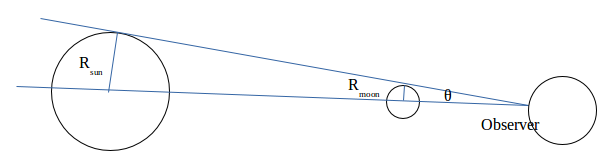
\includegraphics[width=0.7\textwidth]{gambar/osk2016_21.png}
\end{figure}
Untuk sudut kecil berlaku hubungan $\sin{\theta} \approx \tan{\theta} \approx \theta (\text{dalam radian})$. Atau dengan memanfaatkan hubungan kesebangunan, diperoleh
\begin{eqnarray*}
\theta_{\leftmoon} &=& \theta_{\odot}\\
\frac{R_{\leftmoon}}{d_{\text{observer} \leftmoon}} &=& \frac{R_{\odot}}{d_{\text{observer} \odot}} \\
\frac{R_{\leftmoon}}{d_{\text{obs} \leftmoon}} &=& \frac{R_{\odot}}{d_{\oplus \odot} - R_{\oplus}} \\
\frac{1,737 \times 10^{6}}{d_{\text{obs} \leftmoon}} &=& \frac{6,96 \times 10^{8}}{1,49593622 \times 10^{11}}\\
d_{\text{obs} \leftmoon} &=& 373339,254 \quad \text{km}
\end{eqnarray*}


\vspace{0.5cm}
\question Perhatikan gambar berikut ini!
\begin{figure}[H]
\centering
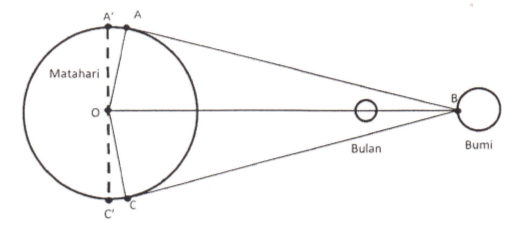
\includegraphics[width=0.7\textwidth]{gambar/osk2016_22.png}
\end{figure}
Gerhana Matahari Total atau Cincin dapat terjadi ketika Bulan memasuki kerucut pandangan ke arah Matahari. Berapakah diameter kerucut tersebut pada radius orbit Bulan?
\begin{choices}
\choice 900 km
\choice 1800 km
\choice 3600 km
\choice 4500 km
\choice 4800 km
\end{choices}

\textit{Jawaban: C}\\
\begin{figure}[H]
\centering
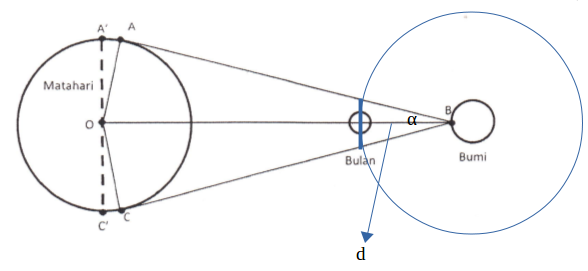
\includegraphics[width=0.7\textwidth]{gambar/osk2016_22b.png}
\end{figure}
Diameter sudut Matahari ($\alpha_{\odot} = 2 \theta_{\odot}$, lihat gambar pada penjelasan nomor 21) dapat dihitung dengan 
\begin{eqnarray*}
\theta_{\odot} &=& \frac{R_{\odot}}{d_{\text{observer} \odot}} = \frac{R_{\odot}}{d_{\oplus \odot} - R_{\oplus}}\\
\theta_{\odot} &=& 0,00465260477 \quad \text{rad} \\
\alpha_{\odot} &=& 2 \times \theta_{\odot} = 0,00930520954 \text{ rad} = 0.53315^{\circ}
\end{eqnarray*}
Diameter kerucut pada radius orbit Bulan dapat ditentukan dengan
\begin{eqnarray*}
D_{\text{kerucut}} &=& \alpha \cdot d_{\text{obs} \leftmoon} = 0,00930520954 \cdot 3,78022\times 10^5\\
&=& 3517,57 \quad \text{km}
\end{eqnarray*}

\vspace{1cm}
\textbf{Gunakan petunjuk ini untuk menjawab soal no. 23-28.}\\
A. jika pernyataan  1, 2, dan 3 benar\\
B. jika pernyataan 1 dan 3 benar\\
C. jika pernyataan 2 dan 4 benar\\
D. jika pernyataan 4 saja benar\\
E. jika semua pernyataan benar\\

\question Suatu eksperimen bola pantul dilakukan di permukaan Bumi dan Bulan. Bola yang identik dijatuhkan secara bebas dari ketinggian yang sama dan dibiarkan memantul di atas lantai beton. Pilihlah pernyataan yang benar berdasarkan eksperimen tersebut!
\begin{enumerate}
\item Pada ketinggian awal yang sama, jarak yang ditempuh sampai bola uji berhenti berbeda untuk Bumi dan Bulan.
\item Pada ketinggian awal yang sama, kecepatan bola saat mencapai tanah sama untuk planet Bumi dan satelit Bulan.
\item Gaya gravitasi bergantung dengan massa benda, sehingga gaya gravitasi yang dialami bola sama.
\item Kecepatan di puncak pantulan untuk bola uji di planet Bumi dan satelit Bulan sama.
\end{enumerate}

\textit{Jawaban: D}\\
Penjelasan untuk masing-masing pernyataan:
\begin{enumerate}
\item Asumsikan eksperimen yang dilakukan di Bumi dilakukan di tempat yang hampa udara (sehampa permukaan Bulan). Bola yang jatuh akan mengalami percepatan ($g$) yang berbeda, sehingga sesampainya di beton, kecepatan bola berbeda pula. 
\begin{eqnarray*}
v^2 &=& v_{0}^2 + 2 g h = 2gh\\
v &=& \sqrt{2gh}
\end{eqnarray*}
Pantulan bola dari beton (koefisien elastisitas/restitusi) hanya bergantung pada material penyusunnya, tidak bergantung pada percepatan gravitasi. Kecepatan setelah tumbukan menjadi
\begin{eqnarray*}
v' = e \cdot v = e \cdot \sqrt{2gh}
\end{eqnarray*}
dan ketinggian setelah tumbukan menjadi
\begin{equation*}
h' = \frac{\frac{1}{2} v'^2}{g} = \frac{\frac{1}{2} \cdot e^2 \cdot 2gh}{g} = e^2 \cdot h
\end{equation*}
Ternyata ketinggian setelah pantulan tidak bergantung pada percepatan gravitasi. Walaupun di Bulan kecepatan bola  saat hampir menumbuk beton lebih kecil, karena percepatan gravitasinya lebih kecil, akan tetapi karena gravitasinya yang kecil itu pula menyebabkan bola dapat memantul lebih tinggi, hingga ketinggian yang sama dengan bola yang di Bumi. Karena ketinggian pantulan sama, maka total lintasan bola sampai berhenti juga akan sama. (Pernyataan 1 \textbf{SALAH})
\item Kecepatan bola saat menyentuh tanah bergantung pada percepatan gravitasi lokal di tempat bola berada. Percepatan gravitasi di Bumi dan Bulan tidak sama, sehingga meski dijatuhkan dari ketinggian yang sama, bola tersebut akan memiliki kecepatan berbeda saat menyentuh tanah. (Pernyataan 2 \textbf{SALAH})
\item Gaya gravitasi bergantung pada massa dan percepatan gravitasi. Dengan massa sama dan percepatan berbeda, gaya gravitasi yang dialami bola berbeda. (Pernyataan 3 \textbf{SALAH})
\item Kecepatan bola di puncak pantulan selalu = 0. (Pernyataan 4 \textbf{BENAR})
\end{enumerate}


\question Pilihlah pernyataan yang benar tentang hukum gravitasi Newton!
\begin{enumerate}
\item Gaya yang bekerja pada koin yang jatuh bebas dan gaya yang menyebabkan Bulan mengitari Bumi adalah gaya gravitasi.
\item Gaya yang menghambat gerak pesawat saat lepas landas dan yang menyebabkan meteoroid mengitari Bumi adalah gaya gravitasi. 
\item Hukum gravitasi Newton dapat membuktikan Hukum III Kepler.
\item Hukum gravitasi membuktikan teori Bohr tentang gerak elektron yang mirip dengan gerak planet.
\end{enumerate}

\textit{Jawaban: A}\\
Penjelasan untuk masing-masing pernyataan:
\begin{enumerate}
\item Gaya gravitasi menyebabkan koin jatuh ke permukaan Bumi, gaya gravitasi pula yang mengikat Bulan mengitari Bumi (Bulan sebetulnya juga selalu jatuh ke Bumi). (\textbf{Pernyataan 1 BENAR})
\item Gravitasi Bumi memberi perlambatan (menghambat) pada gerak pesawat saat lepas landas (gerakan naik), gravitasi pula yang menyebabkan sebagian meteoroid bergerak mengitari Bumi. (\textbf{Pernyataan 2 BENAR})

Pernyataan ini masih ambigu, karena bisa diartikan bukan gaya gravitasi melainkan gaya gesek udara yang menghambat gerak pesawat, dan tentu gaya gesek udara tidak menyebabkan meteoroid mengitari Bumi. 
\item Hukum III Kepler dapat diturunkan dari hukum gravitasi Newton pada sistem 2 benda yang saling mengitari. (\textbf{Pernyataan 3 BENAR})
\item Gerak elektron mengelilingi inti atom bukan diatur oleh gaya gravitasi. Gravitasi antara elektron dan proton jauh lebih kecil dibandingkan gaya Coulomb antara keduanya. Elektron memiliki tingkat energi diskrit yang memungkinkan mereka `bergerak mengelilingi inti' atom pada jarak berbeda-beda. (\textbf{Pernyataan 4 SALAH})
\end{enumerate}

\question Masyarakat di kota-kota berikut ini dapat mengamati Gerhana Matahari Total yang akan terjadi pada bulan Maret 2016.
\begin{enumerate}
\item Palembang (Sumatera Selatan)
\item Sofifi (Maluku Utara)
\item Palangkaraya (Kalimantan Tengah)
\item Pontianak (Kalimantan Barat)
\end{enumerate}

\textit{Jawaban: A}\\
Lihat \href{http://xjubier.free.fr/en/site_pages/solar_eclipses/TSE_2016_GoogleMapFull.html}
{peta jalur Gerhana Matahari Total 9 Maret 2016}. Dari keempat kota tersebut hanya Pontianak yang mengalami gerhana Matahari sebagian. Sofifi adalah ibukota Provinsi Maluku Utara, pengganti Ternate (catatan untuk penulis).

$^{\star\star}$Sebelum olimpiade rajinlah membaca berita atau \textit{event} astronomi terkini. 


\question Gambar di bawah ini menunjukkan tiga posisi \textit{landrover} yang menjalajahi pegunungan bersalju di planet Mars.
\begin{figure}[H]
\centering
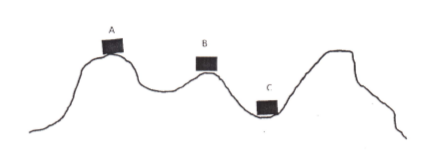
\includegraphics[width=0.7\textwidth]{gambar/osk2016_26.png}
\end{figure}
Diawali dari posisi puncak A, \textit{landrover} meluncur bebas melewati titik B dan C. Asumsikan tidak ada gesekan dan faktor eksternal yang mempengaruhi \textit{landrover}. Pilih pernyataan yang benar!
\begin{enumerate}
\item Energi potensial B lebih rendah daripada energi potensial di C.
\item Energi mekanik C sama dengan energi potensial A.
\item Energi kinetik C lebih rendah dari energi potensial B.
\item Energi mekanik di semua posisi tetap.
\end{enumerate}

\textit{Jawaban: C}\\
Penjelasan untuk masing-masing pernyataan:
\begin{enumerate}
\item Posisi yang lebih tinggi memiliki nilai energi potensial lebih besar. B lebih tinggi daripada C, sehingga energi potensial di B lebih tinggi daripada energi potensial di C. (Pernyataan 1 \textbf{SALAH})
\item Energi total mekanik dalam sistem tersebut selalu kekal. Di A, mula-mula energi kinetik bernilai nol (terdapat kata-kata ``meluncur bebas'') sehingga nilai energi total mekanik sama dengan nilai energi potensial di titik A. (Pernyataan 2 \textbf{BENAR})
\item Dengan nilai energi total mekanik selalu tetap dan energi potensial di B lebih rendah daripada energi potensial di C, maka energi kinetik di C lebih tinggi daripada energi kinetik di B. Dari gambar tersebut, di antara titik A, B, dan C, titik C merupakan titik terendah sehingga jika memang tidak ada titik yang lebih rendah daripada C yang dilewati oleh \textit{landrover}, dapat dipastikan energi kinetik di C sama dengan energi potensial di A. Padahal energi potensial di A lebih besar daripada energi potensial di B. Sehingga energi kinetik di C harus lebih besar daripada energi potensial di B. (Pernyataan 3 \textbf{SALAH})
\item Energi mekanik di semua posisi dalam sistem itu tetap. (Pernyataan 4 \textbf{BENAR})
\end{enumerate}

\question Kemajuan teknologi di masa kini memberikan harapan bagi manusia untuk migrasi ke planet lain. Anggap di masa depan manusia telah berhasil membuat koloni di Mars. Pernyataan yang benar adalah
\begin{enumerate}
\item Definisi 1 parsek tetap sebesar 206265 au (atau 206265 sa).
\item Peristiwa konjungsi inferior lebih jarang terjadi. 
\item Terdapat pembagian musim menurut lintang di Mars.
\item Tidak ada perubahan musim di Mars.
\end{enumerate}

\textit{Jawaban: B}\\
Penjelasan untuk masing-masing pernyataan:
\begin{enumerate}
\item Definisi 1 parsek tetap atau tidak tentu bergantung kepada manusia saat itu. Jika masih menyepakati definisi satu parsek yang sekarang, ``Wikipedia: \textit{One parsec is the distance at which one astronomical unit subtends an angle of one arcsecond}'', maka sudah sewajarnya akan tetap sebesar 206265 sa. (Pernyataan 1 \textbf{BENAR})
\item Peristiwa konjungsi inferior akan lebih sering terjadi karena ada tiga planet yang mungkin mengalami konjungsi inferior dilihat dari Mars (Merkurius, Venus, dan Bumi). (Pernyataan 2 \textbf{SALAH})
\item Pembagian musim di Mars bisa ditentukan bahkan sebelum manusia membuat koloni di Mars (perbedaan musim terjadi karena kemiringan sumbu rotasi Mars terhadap ekliptika). Adanya koloni meningkatkan kemungkinan penentuan musim menurut lintang secara lebih spesifik. (Pernyataan 3 \textbf{BENAR})
\item Perubahan musim terjadi di Mars. (Pernyataan 4 \textbf{SALAH})

\end{enumerate}

\question Berikut ini merupakan pernyataan-pernyataan mengenai gerhana. Pernyataan yang benar adalah
\begin{enumerate}
\item Gerhana Matahari Total hanya dapat diamati pada ruang lingkup yang sempit di Bumi.
\item Gerhana Matahari dan gerhana Bulan dapat dilihat di seluruh permukaan Bumi.
\item Gerhana Bulan dapat diamati di hampir seluruh wilayah malam di Bumi.
\item Gerhana Matahari lebih jarang terjadi dibanding gerhana Bulan.
\end{enumerate}

\textit{Jawaban: B}\\
Penjelasan untuk masing-masing pernyataan:
\begin{enumerate}
\item Ukuran umbra Bulan yang jatuh di permukaan Bumi relatif kecil, sehingga Gerhana Matahari Total hanya dapat diamati pada ruang lingkup yang sempit di Bumi. (Pernyataan 1 \textbf{BENAR})
\item Gerhana Matahari maupun gerhana Bulan tidak dapat dilihat di seluruh permukaan Bumi. (Pernyataan 2 \textbf{SALAH})
\item Seluruh wilayah yang sedang mengalami malam dapat mengamati peristiwa gerhana bulan. (Pernyataan 3 \textbf{BENAR})
\item Gerhana Matahari lebih sering terjadi dibanding gerhana Bulan, tetapi lebih jarang diamati karena hanya melingkupi kawasan yang sempit dan kebanyakan permukaan Bumi merupakan lautan yang tidak dihuni manusia. (Pernyataan 4 \textbf{SALAH})
\end{enumerate}

\textbf{Gunakan petunjuk ini untuk menjawab soal no. 29-30.}\\
A. Pernyataan pertama dan kedua benar serta memiliki hubungan sebab-akibat.\\
B. Pernyataan pertama dan kedua benar, tetapi tidak memiliki hubungan sebab-akibat.\\
C. Pernyataan pertama benar, sedangkan pernyataan kedua salah.\\
D. Pernyataan pertama salah, sedangkan pernyataan kedua benar\\
E. Kedua pernyataan salah.\\

\question Last year, Pluto became a trending topic in the news as a space craft named Dawn visited this freezing cold body of Solar System. Since 2006, Pluto has been defined as dwarf planet.
\begin{center}
BECAUSE
\end{center}
\noindent This rocky planet has more than one satellite differs from other terrestrial planets such as Earth.

\textit{Jawaban: E}\\
Pluto has been defined as dwarf planet since 2006. It was New Horizons, not Dawn, that visited Pluto last year. (\textbf{Pernyataan pertama SALAH})


Pluto has at least 5 satellites around it. It is highlighted that Pluto is not a planet, but a dwarf planet. The beginning of the second statement: ``This rocky planet ...'' is not valid. Mars as terrestrial planet has more than one satellite: Phobos and Deimos. (\textbf{Pernyataan kedua SALAH})

\question Terdapat dua bintang identik pada jarak yang sama, tetapi salah satu bintang berada di bidang Galaksi sedangkan yang lain berada di atas bidang Galaksi. Bintang yang berada di bidang Galaksi tampak lebih merah dibandingkan bintang kedua. 
\begin{center}
SEBAB
\end{center}
\noindent Di bidang Galaksi, terdapat gas antarbintang dengan kerapatan yang sama seperti atmosfer Bumi. Gas tersebut membuat bintang tampak lebih merah sebagaimana halnya atmosfer Bumi memerahkan Matahari di kala senja.

\textit{Jawaban: C}\\
Materi antarbintang menyebabkan efek pemerahan pada bintang, foton berpanjang gelombang biru dihamburkan lebih banyak daripada foton berpanjang gelombang merah, sehingga foton dengan panjang gelombang merah diteruskan lebih banyak ke pengamat. Jika dua bintang identik (terang dan warna sebenarnya sama) berada pada jarak yang sama, maka bintang yang berada di bidang galaksi akan tampak lebih merah karena cahayanya melewati gas/materi antarbintang lebih banyak. (\textbf{Pernyataan pertama BENAR})


Proses terjadinya efek pemerahan ini seperti halnya atmosfer Bumi memerahkan Matahari di kala senja. Namun, kerapatan gas antarbintang biasanya jauh lebih rendah dari kerapatan atmosfer Bumi (tidak sama). (\textbf{Pernyataan kedua SALAH})

\end{questions}

\vspace{1cm}
\begin{flushright}
Dapat diperoleh di \href{http://ridlow.wordpress.com}{http://ridlow.wordpress.com}
\end{flushright}
\end{document}
